% Created by tikzDevice version 0.12.6 on 2024-02-26 22:01:50
% !TEX encoding = UTF-8 Unicode
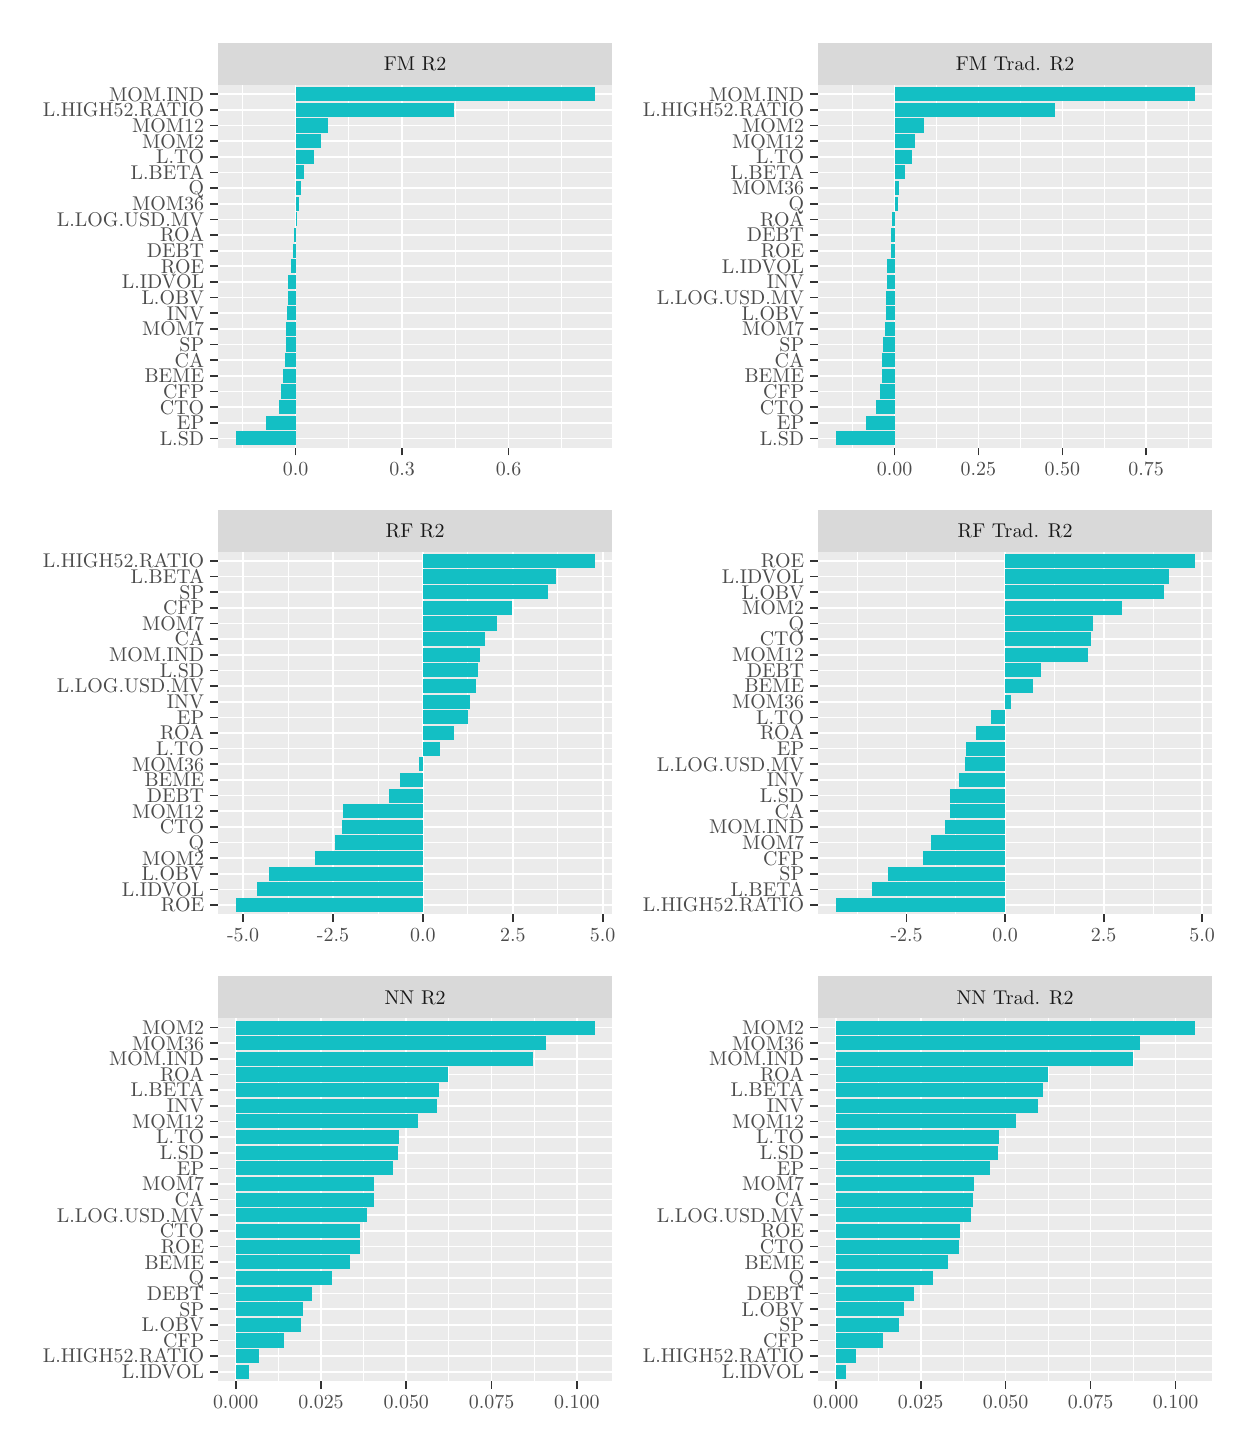
\begin{tikzpicture}[x=1pt,y=1pt]
\definecolor{fillColor}{RGB}{255,255,255}
\path[use as bounding box,fill=fillColor,fill opacity=0.00] (0,0) rectangle (433.62,505.89);
\begin{scope}
\path[clip] (  0.00,337.26) rectangle (216.81,505.89);
\definecolor{drawColor}{RGB}{255,255,255}
\definecolor{fillColor}{RGB}{255,255,255}

\path[draw=drawColor,line width= 0.6pt,line join=round,line cap=round,fill=fillColor] (  0.00,337.26) rectangle (216.81,505.89);
\end{scope}
\begin{scope}
\path[clip] ( 68.69,354.07) rectangle (211.31,485.23);
\definecolor{fillColor}{gray}{0.92}

\path[fill=fillColor] ( 68.69,354.07) rectangle (211.31,485.23);
\definecolor{drawColor}{RGB}{255,255,255}

\path[draw=drawColor,line width= 0.3pt,line join=round] ( 77.58,354.07) --
	( 77.58,485.23);

\path[draw=drawColor,line width= 0.3pt,line join=round] (116.04,354.07) --
	(116.04,485.23);

\path[draw=drawColor,line width= 0.3pt,line join=round] (154.51,354.07) --
	(154.51,485.23);

\path[draw=drawColor,line width= 0.3pt,line join=round] (192.97,354.07) --
	(192.97,485.23);

\path[draw=drawColor,line width= 0.6pt,line join=round] ( 68.69,357.46) --
	(211.31,357.46);

\path[draw=drawColor,line width= 0.6pt,line join=round] ( 68.69,363.11) --
	(211.31,363.11);

\path[draw=drawColor,line width= 0.6pt,line join=round] ( 68.69,368.77) --
	(211.31,368.77);

\path[draw=drawColor,line width= 0.6pt,line join=round] ( 68.69,374.42) --
	(211.31,374.42);

\path[draw=drawColor,line width= 0.6pt,line join=round] ( 68.69,380.07) --
	(211.31,380.07);

\path[draw=drawColor,line width= 0.6pt,line join=round] ( 68.69,385.73) --
	(211.31,385.73);

\path[draw=drawColor,line width= 0.6pt,line join=round] ( 68.69,391.38) --
	(211.31,391.38);

\path[draw=drawColor,line width= 0.6pt,line join=round] ( 68.69,397.04) --
	(211.31,397.04);

\path[draw=drawColor,line width= 0.6pt,line join=round] ( 68.69,402.69) --
	(211.31,402.69);

\path[draw=drawColor,line width= 0.6pt,line join=round] ( 68.69,408.34) --
	(211.31,408.34);

\path[draw=drawColor,line width= 0.6pt,line join=round] ( 68.69,414.00) --
	(211.31,414.00);

\path[draw=drawColor,line width= 0.6pt,line join=round] ( 68.69,419.65) --
	(211.31,419.65);

\path[draw=drawColor,line width= 0.6pt,line join=round] ( 68.69,425.30) --
	(211.31,425.30);

\path[draw=drawColor,line width= 0.6pt,line join=round] ( 68.69,430.96) --
	(211.31,430.96);

\path[draw=drawColor,line width= 0.6pt,line join=round] ( 68.69,436.61) --
	(211.31,436.61);

\path[draw=drawColor,line width= 0.6pt,line join=round] ( 68.69,442.26) --
	(211.31,442.26);

\path[draw=drawColor,line width= 0.6pt,line join=round] ( 68.69,447.92) --
	(211.31,447.92);

\path[draw=drawColor,line width= 0.6pt,line join=round] ( 68.69,453.57) --
	(211.31,453.57);

\path[draw=drawColor,line width= 0.6pt,line join=round] ( 68.69,459.23) --
	(211.31,459.23);

\path[draw=drawColor,line width= 0.6pt,line join=round] ( 68.69,464.88) --
	(211.31,464.88);

\path[draw=drawColor,line width= 0.6pt,line join=round] ( 68.69,470.53) --
	(211.31,470.53);

\path[draw=drawColor,line width= 0.6pt,line join=round] ( 68.69,476.19) --
	(211.31,476.19);

\path[draw=drawColor,line width= 0.6pt,line join=round] ( 68.69,481.84) --
	(211.31,481.84);

\path[draw=drawColor,line width= 0.6pt,line join=round] ( 96.81,354.07) --
	( 96.81,485.23);

\path[draw=drawColor,line width= 0.6pt,line join=round] (135.27,354.07) --
	(135.27,485.23);

\path[draw=drawColor,line width= 0.6pt,line join=round] (173.74,354.07) --
	(173.74,485.23);
\definecolor{fillColor}{RGB}{19,191,196}

\path[fill=fillColor] ( 92.99,383.18) rectangle ( 96.81,388.27);

\path[fill=fillColor] ( 90.67,366.22) rectangle ( 96.81,371.31);

\path[fill=fillColor] ( 92.16,377.53) rectangle ( 96.81,382.62);

\path[fill=fillColor] ( 91.63,371.88) rectangle ( 96.81,376.97);

\path[fill=fillColor] ( 93.83,400.15) rectangle ( 96.81,405.23);

\path[fill=fillColor] ( 95.85,422.76) rectangle ( 96.81,427.85);

\path[fill=fillColor] ( 93.18,388.84) rectangle ( 96.81,393.93);

\path[fill=fillColor] ( 86.09,360.57) rectangle ( 96.81,365.66);

\path[fill=fillColor] ( 96.10,428.41) rectangle ( 96.81,433.50);

\path[fill=fillColor] ( 95.28,417.11) rectangle ( 96.81,422.19);

\path[fill=fillColor] ( 96.81,445.37) rectangle ( 98.61,450.46);

\path[fill=fillColor] ( 93.47,394.49) rectangle ( 96.81,399.58);

\path[fill=fillColor] ( 96.81,467.99) rectangle (108.56,473.08);

\path[fill=fillColor] ( 96.81,439.72) rectangle ( 98.07,444.81);

\path[fill=fillColor] ( 96.81,462.33) rectangle (105.85,467.42);

\path[fill=fillColor] ( 96.81,479.30) rectangle (204.83,484.38);

\path[fill=fillColor] ( 75.17,354.92) rectangle ( 96.81,360.00);

\path[fill=fillColor] ( 96.81,473.64) rectangle (154.00,478.73);

\path[fill=fillColor] ( 96.81,451.03) rectangle ( 99.97,456.12);

\path[fill=fillColor] ( 94.19,411.45) rectangle ( 96.81,416.54);

\path[fill=fillColor] ( 96.81,434.07) rectangle ( 96.88,439.15);

\path[fill=fillColor] ( 96.81,456.68) rectangle (103.55,461.77);

\path[fill=fillColor] ( 93.92,405.80) rectangle ( 96.81,410.89);
\end{scope}
\begin{scope}
\path[clip] ( 68.69,485.23) rectangle (211.31,500.39);
\definecolor{fillColor}{gray}{0.85}

\path[fill=fillColor] ( 68.69,485.23) rectangle (211.31,500.39);
\definecolor{drawColor}{gray}{0.10}

\node[text=drawColor,anchor=base,inner sep=0pt, outer sep=0pt, scale=  0.72] at (140.00,490.33) {FM R2};
\end{scope}
\begin{scope}
\path[clip] (  0.00,  0.00) rectangle (433.62,505.89);
\definecolor{drawColor}{gray}{0.20}

\path[draw=drawColor,line width= 0.6pt,line join=round] ( 96.81,351.32) --
	( 96.81,354.07);

\path[draw=drawColor,line width= 0.6pt,line join=round] (135.27,351.32) --
	(135.27,354.07);

\path[draw=drawColor,line width= 0.6pt,line join=round] (173.74,351.32) --
	(173.74,354.07);
\end{scope}
\begin{scope}
\path[clip] (  0.00,  0.00) rectangle (433.62,505.89);
\definecolor{drawColor}{gray}{0.30}

\node[text=drawColor,anchor=base,inner sep=0pt, outer sep=0pt, scale=  0.72] at ( 96.81,344.16) {0.0};

\node[text=drawColor,anchor=base,inner sep=0pt, outer sep=0pt, scale=  0.72] at (135.27,344.16) {0.3};

\node[text=drawColor,anchor=base,inner sep=0pt, outer sep=0pt, scale=  0.72] at (173.74,344.16) {0.6};
\end{scope}
\begin{scope}
\path[clip] (  0.00,  0.00) rectangle (433.62,505.89);
\definecolor{drawColor}{gray}{0.30}

\node[text=drawColor,anchor=base east,inner sep=0pt, outer sep=0pt, scale=  0.72] at ( 63.74,354.98) {L.SD};

\node[text=drawColor,anchor=base east,inner sep=0pt, outer sep=0pt, scale=  0.72] at ( 63.74,360.63) {EP};

\node[text=drawColor,anchor=base east,inner sep=0pt, outer sep=0pt, scale=  0.72] at ( 63.74,366.29) {CTO};

\node[text=drawColor,anchor=base east,inner sep=0pt, outer sep=0pt, scale=  0.72] at ( 63.74,371.94) {CFP};

\node[text=drawColor,anchor=base east,inner sep=0pt, outer sep=0pt, scale=  0.72] at ( 63.74,377.60) {BEME};

\node[text=drawColor,anchor=base east,inner sep=0pt, outer sep=0pt, scale=  0.72] at ( 63.74,383.25) {CA};

\node[text=drawColor,anchor=base east,inner sep=0pt, outer sep=0pt, scale=  0.72] at ( 63.74,388.90) {SP};

\node[text=drawColor,anchor=base east,inner sep=0pt, outer sep=0pt, scale=  0.72] at ( 63.74,394.56) {MOM7};

\node[text=drawColor,anchor=base east,inner sep=0pt, outer sep=0pt, scale=  0.72] at ( 63.74,400.21) {INV};

\node[text=drawColor,anchor=base east,inner sep=0pt, outer sep=0pt, scale=  0.72] at ( 63.74,405.86) {L.OBV};

\node[text=drawColor,anchor=base east,inner sep=0pt, outer sep=0pt, scale=  0.72] at ( 63.74,411.52) {L.IDVOL};

\node[text=drawColor,anchor=base east,inner sep=0pt, outer sep=0pt, scale=  0.72] at ( 63.74,417.17) {ROE};

\node[text=drawColor,anchor=base east,inner sep=0pt, outer sep=0pt, scale=  0.72] at ( 63.74,422.82) {DEBT};

\node[text=drawColor,anchor=base east,inner sep=0pt, outer sep=0pt, scale=  0.72] at ( 63.74,428.48) {ROA};

\node[text=drawColor,anchor=base east,inner sep=0pt, outer sep=0pt, scale=  0.72] at ( 63.74,434.13) {L.LOG.USD.MV};

\node[text=drawColor,anchor=base east,inner sep=0pt, outer sep=0pt, scale=  0.72] at ( 63.74,439.78) {MOM36};

\node[text=drawColor,anchor=base east,inner sep=0pt, outer sep=0pt, scale=  0.72] at ( 63.74,445.44) {Q};

\node[text=drawColor,anchor=base east,inner sep=0pt, outer sep=0pt, scale=  0.72] at ( 63.74,451.09) {L.BETA};

\node[text=drawColor,anchor=base east,inner sep=0pt, outer sep=0pt, scale=  0.72] at ( 63.74,456.75) {L.TO};

\node[text=drawColor,anchor=base east,inner sep=0pt, outer sep=0pt, scale=  0.72] at ( 63.74,462.40) {MOM2};

\node[text=drawColor,anchor=base east,inner sep=0pt, outer sep=0pt, scale=  0.72] at ( 63.74,468.05) {MOM12};

\node[text=drawColor,anchor=base east,inner sep=0pt, outer sep=0pt, scale=  0.72] at ( 63.74,473.71) {L.HIGH52.RATIO};

\node[text=drawColor,anchor=base east,inner sep=0pt, outer sep=0pt, scale=  0.72] at ( 63.74,479.36) {MOM.IND};
\end{scope}
\begin{scope}
\path[clip] (  0.00,  0.00) rectangle (433.62,505.89);
\definecolor{drawColor}{gray}{0.20}

\path[draw=drawColor,line width= 0.6pt,line join=round] ( 65.94,357.46) --
	( 68.69,357.46);

\path[draw=drawColor,line width= 0.6pt,line join=round] ( 65.94,363.11) --
	( 68.69,363.11);

\path[draw=drawColor,line width= 0.6pt,line join=round] ( 65.94,368.77) --
	( 68.69,368.77);

\path[draw=drawColor,line width= 0.6pt,line join=round] ( 65.94,374.42) --
	( 68.69,374.42);

\path[draw=drawColor,line width= 0.6pt,line join=round] ( 65.94,380.07) --
	( 68.69,380.07);

\path[draw=drawColor,line width= 0.6pt,line join=round] ( 65.94,385.73) --
	( 68.69,385.73);

\path[draw=drawColor,line width= 0.6pt,line join=round] ( 65.94,391.38) --
	( 68.69,391.38);

\path[draw=drawColor,line width= 0.6pt,line join=round] ( 65.94,397.04) --
	( 68.69,397.04);

\path[draw=drawColor,line width= 0.6pt,line join=round] ( 65.94,402.69) --
	( 68.69,402.69);

\path[draw=drawColor,line width= 0.6pt,line join=round] ( 65.94,408.34) --
	( 68.69,408.34);

\path[draw=drawColor,line width= 0.6pt,line join=round] ( 65.94,414.00) --
	( 68.69,414.00);

\path[draw=drawColor,line width= 0.6pt,line join=round] ( 65.94,419.65) --
	( 68.69,419.65);

\path[draw=drawColor,line width= 0.6pt,line join=round] ( 65.94,425.30) --
	( 68.69,425.30);

\path[draw=drawColor,line width= 0.6pt,line join=round] ( 65.94,430.96) --
	( 68.69,430.96);

\path[draw=drawColor,line width= 0.6pt,line join=round] ( 65.94,436.61) --
	( 68.69,436.61);

\path[draw=drawColor,line width= 0.6pt,line join=round] ( 65.94,442.26) --
	( 68.69,442.26);

\path[draw=drawColor,line width= 0.6pt,line join=round] ( 65.94,447.92) --
	( 68.69,447.92);

\path[draw=drawColor,line width= 0.6pt,line join=round] ( 65.94,453.57) --
	( 68.69,453.57);

\path[draw=drawColor,line width= 0.6pt,line join=round] ( 65.94,459.23) --
	( 68.69,459.23);

\path[draw=drawColor,line width= 0.6pt,line join=round] ( 65.94,464.88) --
	( 68.69,464.88);

\path[draw=drawColor,line width= 0.6pt,line join=round] ( 65.94,470.53) --
	( 68.69,470.53);

\path[draw=drawColor,line width= 0.6pt,line join=round] ( 65.94,476.19) --
	( 68.69,476.19);

\path[draw=drawColor,line width= 0.6pt,line join=round] ( 65.94,481.84) --
	( 68.69,481.84);
\end{scope}
\begin{scope}
\path[clip] (216.81,337.26) rectangle (433.62,505.89);
\definecolor{drawColor}{RGB}{255,255,255}
\definecolor{fillColor}{RGB}{255,255,255}

\path[draw=drawColor,line width= 0.6pt,line join=round,line cap=round,fill=fillColor] (216.81,337.26) rectangle (433.62,505.89);
\end{scope}
\begin{scope}
\path[clip] (285.50,354.07) rectangle (428.12,485.23);
\definecolor{fillColor}{gray}{0.92}

\path[fill=fillColor] (285.50,354.07) rectangle (428.12,485.23);
\definecolor{drawColor}{RGB}{255,255,255}

\path[draw=drawColor,line width= 0.3pt,line join=round] (298.10,354.07) --
	(298.10,485.23);

\path[draw=drawColor,line width= 0.3pt,line join=round] (328.41,354.07) --
	(328.41,485.23);

\path[draw=drawColor,line width= 0.3pt,line join=round] (358.72,354.07) --
	(358.72,485.23);

\path[draw=drawColor,line width= 0.3pt,line join=round] (389.03,354.07) --
	(389.03,485.23);

\path[draw=drawColor,line width= 0.3pt,line join=round] (419.33,354.07) --
	(419.33,485.23);

\path[draw=drawColor,line width= 0.6pt,line join=round] (285.50,357.46) --
	(428.12,357.46);

\path[draw=drawColor,line width= 0.6pt,line join=round] (285.50,363.11) --
	(428.12,363.11);

\path[draw=drawColor,line width= 0.6pt,line join=round] (285.50,368.77) --
	(428.12,368.77);

\path[draw=drawColor,line width= 0.6pt,line join=round] (285.50,374.42) --
	(428.12,374.42);

\path[draw=drawColor,line width= 0.6pt,line join=round] (285.50,380.07) --
	(428.12,380.07);

\path[draw=drawColor,line width= 0.6pt,line join=round] (285.50,385.73) --
	(428.12,385.73);

\path[draw=drawColor,line width= 0.6pt,line join=round] (285.50,391.38) --
	(428.12,391.38);

\path[draw=drawColor,line width= 0.6pt,line join=round] (285.50,397.04) --
	(428.12,397.04);

\path[draw=drawColor,line width= 0.6pt,line join=round] (285.50,402.69) --
	(428.12,402.69);

\path[draw=drawColor,line width= 0.6pt,line join=round] (285.50,408.34) --
	(428.12,408.34);

\path[draw=drawColor,line width= 0.6pt,line join=round] (285.50,414.00) --
	(428.12,414.00);

\path[draw=drawColor,line width= 0.6pt,line join=round] (285.50,419.65) --
	(428.12,419.65);

\path[draw=drawColor,line width= 0.6pt,line join=round] (285.50,425.30) --
	(428.12,425.30);

\path[draw=drawColor,line width= 0.6pt,line join=round] (285.50,430.96) --
	(428.12,430.96);

\path[draw=drawColor,line width= 0.6pt,line join=round] (285.50,436.61) --
	(428.12,436.61);

\path[draw=drawColor,line width= 0.6pt,line join=round] (285.50,442.26) --
	(428.12,442.26);

\path[draw=drawColor,line width= 0.6pt,line join=round] (285.50,447.92) --
	(428.12,447.92);

\path[draw=drawColor,line width= 0.6pt,line join=round] (285.50,453.57) --
	(428.12,453.57);

\path[draw=drawColor,line width= 0.6pt,line join=round] (285.50,459.23) --
	(428.12,459.23);

\path[draw=drawColor,line width= 0.6pt,line join=round] (285.50,464.88) --
	(428.12,464.88);

\path[draw=drawColor,line width= 0.6pt,line join=round] (285.50,470.53) --
	(428.12,470.53);

\path[draw=drawColor,line width= 0.6pt,line join=round] (285.50,476.19) --
	(428.12,476.19);

\path[draw=drawColor,line width= 0.6pt,line join=round] (285.50,481.84) --
	(428.12,481.84);

\path[draw=drawColor,line width= 0.6pt,line join=round] (313.25,354.07) --
	(313.25,485.23);

\path[draw=drawColor,line width= 0.6pt,line join=round] (343.56,354.07) --
	(343.56,485.23);

\path[draw=drawColor,line width= 0.6pt,line join=round] (373.87,354.07) --
	(373.87,485.23);

\path[draw=drawColor,line width= 0.6pt,line join=round] (404.18,354.07) --
	(404.18,485.23);
\definecolor{fillColor}{RGB}{19,191,196}

\path[fill=fillColor] (308.74,383.18) rectangle (313.25,388.27);

\path[fill=fillColor] (306.55,366.22) rectangle (313.25,371.31);

\path[fill=fillColor] (308.57,377.53) rectangle (313.25,382.62);

\path[fill=fillColor] (308.11,371.88) rectangle (313.25,376.97);

\path[fill=fillColor] (310.34,411.45) rectangle (313.25,416.54);

\path[fill=fillColor] (311.81,428.41) rectangle (313.25,433.50);

\path[fill=fillColor] (309.12,388.84) rectangle (313.25,393.93);

\path[fill=fillColor] (302.89,360.57) rectangle (313.25,365.66);

\path[fill=fillColor] (312.50,434.07) rectangle (313.25,439.15);

\path[fill=fillColor] (311.79,422.76) rectangle (313.25,427.85);

\path[fill=fillColor] (313.25,439.72) rectangle (314.60,444.81);

\path[fill=fillColor] (309.72,394.49) rectangle (313.25,399.58);

\path[fill=fillColor] (313.25,462.33) rectangle (320.46,467.42);

\path[fill=fillColor] (313.25,445.37) rectangle (314.94,450.46);

\path[fill=fillColor] (313.25,467.99) rectangle (323.93,473.08);

\path[fill=fillColor] (313.25,479.30) rectangle (421.64,484.38);

\path[fill=fillColor] (291.98,354.92) rectangle (313.25,360.00);

\path[fill=fillColor] (313.25,473.64) rectangle (371.08,478.73);

\path[fill=fillColor] (313.25,451.03) rectangle (316.92,456.12);

\path[fill=fillColor] (310.45,417.11) rectangle (313.25,422.19);

\path[fill=fillColor] (310.28,405.80) rectangle (313.25,410.89);

\path[fill=fillColor] (313.25,456.68) rectangle (319.42,461.77);

\path[fill=fillColor] (310.23,400.15) rectangle (313.25,405.23);
\end{scope}
\begin{scope}
\path[clip] (285.50,485.23) rectangle (428.12,500.39);
\definecolor{fillColor}{gray}{0.85}

\path[fill=fillColor] (285.50,485.23) rectangle (428.12,500.39);
\definecolor{drawColor}{gray}{0.10}

\node[text=drawColor,anchor=base,inner sep=0pt, outer sep=0pt, scale=  0.72] at (356.81,490.33) {FM Trad. R2};
\end{scope}
\begin{scope}
\path[clip] (  0.00,  0.00) rectangle (433.62,505.89);
\definecolor{drawColor}{gray}{0.20}

\path[draw=drawColor,line width= 0.6pt,line join=round] (313.25,351.32) --
	(313.25,354.07);

\path[draw=drawColor,line width= 0.6pt,line join=round] (343.56,351.32) --
	(343.56,354.07);

\path[draw=drawColor,line width= 0.6pt,line join=round] (373.87,351.32) --
	(373.87,354.07);

\path[draw=drawColor,line width= 0.6pt,line join=round] (404.18,351.32) --
	(404.18,354.07);
\end{scope}
\begin{scope}
\path[clip] (  0.00,  0.00) rectangle (433.62,505.89);
\definecolor{drawColor}{gray}{0.30}

\node[text=drawColor,anchor=base,inner sep=0pt, outer sep=0pt, scale=  0.72] at (313.25,344.16) {0.00};

\node[text=drawColor,anchor=base,inner sep=0pt, outer sep=0pt, scale=  0.72] at (343.56,344.16) {0.25};

\node[text=drawColor,anchor=base,inner sep=0pt, outer sep=0pt, scale=  0.72] at (373.87,344.16) {0.50};

\node[text=drawColor,anchor=base,inner sep=0pt, outer sep=0pt, scale=  0.72] at (404.18,344.16) {0.75};
\end{scope}
\begin{scope}
\path[clip] (  0.00,  0.00) rectangle (433.62,505.89);
\definecolor{drawColor}{gray}{0.30}

\node[text=drawColor,anchor=base east,inner sep=0pt, outer sep=0pt, scale=  0.72] at (280.55,354.98) {L.SD};

\node[text=drawColor,anchor=base east,inner sep=0pt, outer sep=0pt, scale=  0.72] at (280.55,360.63) {EP};

\node[text=drawColor,anchor=base east,inner sep=0pt, outer sep=0pt, scale=  0.72] at (280.55,366.29) {CTO};

\node[text=drawColor,anchor=base east,inner sep=0pt, outer sep=0pt, scale=  0.72] at (280.55,371.94) {CFP};

\node[text=drawColor,anchor=base east,inner sep=0pt, outer sep=0pt, scale=  0.72] at (280.55,377.60) {BEME};

\node[text=drawColor,anchor=base east,inner sep=0pt, outer sep=0pt, scale=  0.72] at (280.55,383.25) {CA};

\node[text=drawColor,anchor=base east,inner sep=0pt, outer sep=0pt, scale=  0.72] at (280.55,388.90) {SP};

\node[text=drawColor,anchor=base east,inner sep=0pt, outer sep=0pt, scale=  0.72] at (280.55,394.56) {MOM7};

\node[text=drawColor,anchor=base east,inner sep=0pt, outer sep=0pt, scale=  0.72] at (280.55,400.21) {L.OBV};

\node[text=drawColor,anchor=base east,inner sep=0pt, outer sep=0pt, scale=  0.72] at (280.55,405.86) {L.LOG.USD.MV};

\node[text=drawColor,anchor=base east,inner sep=0pt, outer sep=0pt, scale=  0.72] at (280.55,411.52) {INV};

\node[text=drawColor,anchor=base east,inner sep=0pt, outer sep=0pt, scale=  0.72] at (280.55,417.17) {L.IDVOL};

\node[text=drawColor,anchor=base east,inner sep=0pt, outer sep=0pt, scale=  0.72] at (280.55,422.82) {ROE};

\node[text=drawColor,anchor=base east,inner sep=0pt, outer sep=0pt, scale=  0.72] at (280.55,428.48) {DEBT};

\node[text=drawColor,anchor=base east,inner sep=0pt, outer sep=0pt, scale=  0.72] at (280.55,434.13) {ROA};

\node[text=drawColor,anchor=base east,inner sep=0pt, outer sep=0pt, scale=  0.72] at (280.55,439.78) {Q};

\node[text=drawColor,anchor=base east,inner sep=0pt, outer sep=0pt, scale=  0.72] at (280.55,445.44) {MOM36};

\node[text=drawColor,anchor=base east,inner sep=0pt, outer sep=0pt, scale=  0.72] at (280.55,451.09) {L.BETA};

\node[text=drawColor,anchor=base east,inner sep=0pt, outer sep=0pt, scale=  0.72] at (280.55,456.75) {L.TO};

\node[text=drawColor,anchor=base east,inner sep=0pt, outer sep=0pt, scale=  0.72] at (280.55,462.40) {MOM12};

\node[text=drawColor,anchor=base east,inner sep=0pt, outer sep=0pt, scale=  0.72] at (280.55,468.05) {MOM2};

\node[text=drawColor,anchor=base east,inner sep=0pt, outer sep=0pt, scale=  0.72] at (280.55,473.71) {L.HIGH52.RATIO};

\node[text=drawColor,anchor=base east,inner sep=0pt, outer sep=0pt, scale=  0.72] at (280.55,479.36) {MOM.IND};
\end{scope}
\begin{scope}
\path[clip] (  0.00,  0.00) rectangle (433.62,505.89);
\definecolor{drawColor}{gray}{0.20}

\path[draw=drawColor,line width= 0.6pt,line join=round] (282.75,357.46) --
	(285.50,357.46);

\path[draw=drawColor,line width= 0.6pt,line join=round] (282.75,363.11) --
	(285.50,363.11);

\path[draw=drawColor,line width= 0.6pt,line join=round] (282.75,368.77) --
	(285.50,368.77);

\path[draw=drawColor,line width= 0.6pt,line join=round] (282.75,374.42) --
	(285.50,374.42);

\path[draw=drawColor,line width= 0.6pt,line join=round] (282.75,380.07) --
	(285.50,380.07);

\path[draw=drawColor,line width= 0.6pt,line join=round] (282.75,385.73) --
	(285.50,385.73);

\path[draw=drawColor,line width= 0.6pt,line join=round] (282.75,391.38) --
	(285.50,391.38);

\path[draw=drawColor,line width= 0.6pt,line join=round] (282.75,397.04) --
	(285.50,397.04);

\path[draw=drawColor,line width= 0.6pt,line join=round] (282.75,402.69) --
	(285.50,402.69);

\path[draw=drawColor,line width= 0.6pt,line join=round] (282.75,408.34) --
	(285.50,408.34);

\path[draw=drawColor,line width= 0.6pt,line join=round] (282.75,414.00) --
	(285.50,414.00);

\path[draw=drawColor,line width= 0.6pt,line join=round] (282.75,419.65) --
	(285.50,419.65);

\path[draw=drawColor,line width= 0.6pt,line join=round] (282.75,425.30) --
	(285.50,425.30);

\path[draw=drawColor,line width= 0.6pt,line join=round] (282.75,430.96) --
	(285.50,430.96);

\path[draw=drawColor,line width= 0.6pt,line join=round] (282.75,436.61) --
	(285.50,436.61);

\path[draw=drawColor,line width= 0.6pt,line join=round] (282.75,442.26) --
	(285.50,442.26);

\path[draw=drawColor,line width= 0.6pt,line join=round] (282.75,447.92) --
	(285.50,447.92);

\path[draw=drawColor,line width= 0.6pt,line join=round] (282.75,453.57) --
	(285.50,453.57);

\path[draw=drawColor,line width= 0.6pt,line join=round] (282.75,459.23) --
	(285.50,459.23);

\path[draw=drawColor,line width= 0.6pt,line join=round] (282.75,464.88) --
	(285.50,464.88);

\path[draw=drawColor,line width= 0.6pt,line join=round] (282.75,470.53) --
	(285.50,470.53);

\path[draw=drawColor,line width= 0.6pt,line join=round] (282.75,476.19) --
	(285.50,476.19);

\path[draw=drawColor,line width= 0.6pt,line join=round] (282.75,481.84) --
	(285.50,481.84);
\end{scope}
\begin{scope}
\path[clip] (  0.00,168.63) rectangle (216.81,337.26);
\definecolor{drawColor}{RGB}{255,255,255}
\definecolor{fillColor}{RGB}{255,255,255}

\path[draw=drawColor,line width= 0.6pt,line join=round,line cap=round,fill=fillColor] (  0.00,168.63) rectangle (216.81,337.26);
\end{scope}
\begin{scope}
\path[clip] ( 68.69,185.44) rectangle (211.31,316.60);
\definecolor{fillColor}{gray}{0.92}

\path[fill=fillColor] ( 68.69,185.44) rectangle (211.31,316.60);
\definecolor{drawColor}{RGB}{255,255,255}

\path[draw=drawColor,line width= 0.3pt,line join=round] ( 94.09,185.44) --
	( 94.09,316.60);

\path[draw=drawColor,line width= 0.3pt,line join=round] (126.57,185.44) --
	(126.57,316.60);

\path[draw=drawColor,line width= 0.3pt,line join=round] (159.06,185.44) --
	(159.06,316.60);

\path[draw=drawColor,line width= 0.3pt,line join=round] (191.54,185.44) --
	(191.54,316.60);

\path[draw=drawColor,line width= 0.6pt,line join=round] ( 68.69,188.83) --
	(211.31,188.83);

\path[draw=drawColor,line width= 0.6pt,line join=round] ( 68.69,194.48) --
	(211.31,194.48);

\path[draw=drawColor,line width= 0.6pt,line join=round] ( 68.69,200.14) --
	(211.31,200.14);

\path[draw=drawColor,line width= 0.6pt,line join=round] ( 68.69,205.79) --
	(211.31,205.79);

\path[draw=drawColor,line width= 0.6pt,line join=round] ( 68.69,211.44) --
	(211.31,211.44);

\path[draw=drawColor,line width= 0.6pt,line join=round] ( 68.69,217.10) --
	(211.31,217.10);

\path[draw=drawColor,line width= 0.6pt,line join=round] ( 68.69,222.75) --
	(211.31,222.75);

\path[draw=drawColor,line width= 0.6pt,line join=round] ( 68.69,228.41) --
	(211.31,228.41);

\path[draw=drawColor,line width= 0.6pt,line join=round] ( 68.69,234.06) --
	(211.31,234.06);

\path[draw=drawColor,line width= 0.6pt,line join=round] ( 68.69,239.71) --
	(211.31,239.71);

\path[draw=drawColor,line width= 0.6pt,line join=round] ( 68.69,245.37) --
	(211.31,245.37);

\path[draw=drawColor,line width= 0.6pt,line join=round] ( 68.69,251.02) --
	(211.31,251.02);

\path[draw=drawColor,line width= 0.6pt,line join=round] ( 68.69,256.67) --
	(211.31,256.67);

\path[draw=drawColor,line width= 0.6pt,line join=round] ( 68.69,262.33) --
	(211.31,262.33);

\path[draw=drawColor,line width= 0.6pt,line join=round] ( 68.69,267.98) --
	(211.31,267.98);

\path[draw=drawColor,line width= 0.6pt,line join=round] ( 68.69,273.63) --
	(211.31,273.63);

\path[draw=drawColor,line width= 0.6pt,line join=round] ( 68.69,279.29) --
	(211.31,279.29);

\path[draw=drawColor,line width= 0.6pt,line join=round] ( 68.69,284.94) --
	(211.31,284.94);

\path[draw=drawColor,line width= 0.6pt,line join=round] ( 68.69,290.60) --
	(211.31,290.60);

\path[draw=drawColor,line width= 0.6pt,line join=round] ( 68.69,296.25) --
	(211.31,296.25);

\path[draw=drawColor,line width= 0.6pt,line join=round] ( 68.69,301.90) --
	(211.31,301.90);

\path[draw=drawColor,line width= 0.6pt,line join=round] ( 68.69,307.56) --
	(211.31,307.56);

\path[draw=drawColor,line width= 0.6pt,line join=round] ( 68.69,313.21) --
	(211.31,313.21);

\path[draw=drawColor,line width= 0.6pt,line join=round] ( 77.85,185.44) --
	( 77.85,316.60);

\path[draw=drawColor,line width= 0.6pt,line join=round] (110.33,185.44) --
	(110.33,316.60);

\path[draw=drawColor,line width= 0.6pt,line join=round] (142.82,185.44) --
	(142.82,316.60);

\path[draw=drawColor,line width= 0.6pt,line join=round] (175.30,185.44) --
	(175.30,316.60);

\path[draw=drawColor,line width= 0.6pt,line join=round] (207.79,185.44) --
	(207.79,316.60);
\definecolor{fillColor}{RGB}{19,191,196}

\path[fill=fillColor] (142.82,282.40) rectangle (165.14,287.49);

\path[fill=fillColor] (113.76,214.55) rectangle (142.82,219.64);

\path[fill=fillColor] (134.54,231.52) rectangle (142.82,236.60);

\path[fill=fillColor] (142.82,293.70) rectangle (174.91,298.79);

\path[fill=fillColor] (142.82,259.78) rectangle (159.85,264.87);

\path[fill=fillColor] (130.43,225.86) rectangle (142.82,230.95);

\path[fill=fillColor] (142.82,299.36) rectangle (187.97,304.45);

\path[fill=fillColor] (142.82,254.13) rectangle (159.03,259.22);

\path[fill=fillColor] (142.82,248.48) rectangle (154.23,253.56);

\path[fill=fillColor] ( 75.17,186.29) rectangle (142.82,191.37);

\path[fill=fillColor] (111.07,208.90) rectangle (142.82,213.99);

\path[fill=fillColor] (142.82,288.05) rectangle (169.69,293.14);

\path[fill=fillColor] (114.06,220.21) rectangle (142.82,225.30);

\path[fill=fillColor] (141.29,237.17) rectangle (142.82,242.26);

\path[fill=fillColor] (103.74,203.25) rectangle (142.82,208.34);

\path[fill=fillColor] (142.82,276.74) rectangle (163.31,281.83);

\path[fill=fillColor] (142.82,271.09) rectangle (162.85,276.18);

\path[fill=fillColor] (142.82,310.67) rectangle (204.83,315.75);

\path[fill=fillColor] (142.82,305.01) rectangle (190.75,310.10);

\path[fill=fillColor] ( 82.99,191.94) rectangle (142.82,197.03);

\path[fill=fillColor] (142.82,265.44) rectangle (161.87,270.52);

\path[fill=fillColor] (142.82,242.82) rectangle (148.96,247.91);

\path[fill=fillColor] ( 87.33,197.59) rectangle (142.82,202.68);
\end{scope}
\begin{scope}
\path[clip] ( 68.69,316.60) rectangle (211.31,331.76);
\definecolor{fillColor}{gray}{0.85}

\path[fill=fillColor] ( 68.69,316.60) rectangle (211.31,331.76);
\definecolor{drawColor}{gray}{0.10}

\node[text=drawColor,anchor=base,inner sep=0pt, outer sep=0pt, scale=  0.72] at (140.00,321.70) {RF R2};
\end{scope}
\begin{scope}
\path[clip] (  0.00,  0.00) rectangle (433.62,505.89);
\definecolor{drawColor}{gray}{0.20}

\path[draw=drawColor,line width= 0.6pt,line join=round] ( 77.85,182.69) --
	( 77.85,185.44);

\path[draw=drawColor,line width= 0.6pt,line join=round] (110.33,182.69) --
	(110.33,185.44);

\path[draw=drawColor,line width= 0.6pt,line join=round] (142.82,182.69) --
	(142.82,185.44);

\path[draw=drawColor,line width= 0.6pt,line join=round] (175.30,182.69) --
	(175.30,185.44);

\path[draw=drawColor,line width= 0.6pt,line join=round] (207.79,182.69) --
	(207.79,185.44);
\end{scope}
\begin{scope}
\path[clip] (  0.00,  0.00) rectangle (433.62,505.89);
\definecolor{drawColor}{gray}{0.30}

\node[text=drawColor,anchor=base,inner sep=0pt, outer sep=0pt, scale=  0.72] at ( 77.85,175.53) {-5.0};

\node[text=drawColor,anchor=base,inner sep=0pt, outer sep=0pt, scale=  0.72] at (110.33,175.53) {-2.5};

\node[text=drawColor,anchor=base,inner sep=0pt, outer sep=0pt, scale=  0.72] at (142.82,175.53) {0.0};

\node[text=drawColor,anchor=base,inner sep=0pt, outer sep=0pt, scale=  0.72] at (175.30,175.53) {2.5};

\node[text=drawColor,anchor=base,inner sep=0pt, outer sep=0pt, scale=  0.72] at (207.79,175.53) {5.0};
\end{scope}
\begin{scope}
\path[clip] (  0.00,  0.00) rectangle (433.62,505.89);
\definecolor{drawColor}{gray}{0.30}

\node[text=drawColor,anchor=base east,inner sep=0pt, outer sep=0pt, scale=  0.72] at ( 63.74,186.35) {ROE};

\node[text=drawColor,anchor=base east,inner sep=0pt, outer sep=0pt, scale=  0.72] at ( 63.74,192.00) {L.IDVOL};

\node[text=drawColor,anchor=base east,inner sep=0pt, outer sep=0pt, scale=  0.72] at ( 63.74,197.66) {L.OBV};

\node[text=drawColor,anchor=base east,inner sep=0pt, outer sep=0pt, scale=  0.72] at ( 63.74,203.31) {MOM2};

\node[text=drawColor,anchor=base east,inner sep=0pt, outer sep=0pt, scale=  0.72] at ( 63.74,208.97) {Q};

\node[text=drawColor,anchor=base east,inner sep=0pt, outer sep=0pt, scale=  0.72] at ( 63.74,214.62) {CTO};

\node[text=drawColor,anchor=base east,inner sep=0pt, outer sep=0pt, scale=  0.72] at ( 63.74,220.27) {MOM12};

\node[text=drawColor,anchor=base east,inner sep=0pt, outer sep=0pt, scale=  0.72] at ( 63.74,225.93) {DEBT};

\node[text=drawColor,anchor=base east,inner sep=0pt, outer sep=0pt, scale=  0.72] at ( 63.74,231.58) {BEME};

\node[text=drawColor,anchor=base east,inner sep=0pt, outer sep=0pt, scale=  0.72] at ( 63.74,237.23) {MOM36};

\node[text=drawColor,anchor=base east,inner sep=0pt, outer sep=0pt, scale=  0.72] at ( 63.74,242.89) {L.TO};

\node[text=drawColor,anchor=base east,inner sep=0pt, outer sep=0pt, scale=  0.72] at ( 63.74,248.54) {ROA};

\node[text=drawColor,anchor=base east,inner sep=0pt, outer sep=0pt, scale=  0.72] at ( 63.74,254.19) {EP};

\node[text=drawColor,anchor=base east,inner sep=0pt, outer sep=0pt, scale=  0.72] at ( 63.74,259.85) {INV};

\node[text=drawColor,anchor=base east,inner sep=0pt, outer sep=0pt, scale=  0.72] at ( 63.74,265.50) {L.LOG.USD.MV};

\node[text=drawColor,anchor=base east,inner sep=0pt, outer sep=0pt, scale=  0.72] at ( 63.74,271.15) {L.SD};

\node[text=drawColor,anchor=base east,inner sep=0pt, outer sep=0pt, scale=  0.72] at ( 63.74,276.81) {MOM.IND};

\node[text=drawColor,anchor=base east,inner sep=0pt, outer sep=0pt, scale=  0.72] at ( 63.74,282.46) {CA};

\node[text=drawColor,anchor=base east,inner sep=0pt, outer sep=0pt, scale=  0.72] at ( 63.74,288.12) {MOM7};

\node[text=drawColor,anchor=base east,inner sep=0pt, outer sep=0pt, scale=  0.72] at ( 63.74,293.77) {CFP};

\node[text=drawColor,anchor=base east,inner sep=0pt, outer sep=0pt, scale=  0.72] at ( 63.74,299.42) {SP};

\node[text=drawColor,anchor=base east,inner sep=0pt, outer sep=0pt, scale=  0.72] at ( 63.74,305.08) {L.BETA};

\node[text=drawColor,anchor=base east,inner sep=0pt, outer sep=0pt, scale=  0.72] at ( 63.74,310.73) {L.HIGH52.RATIO};
\end{scope}
\begin{scope}
\path[clip] (  0.00,  0.00) rectangle (433.62,505.89);
\definecolor{drawColor}{gray}{0.20}

\path[draw=drawColor,line width= 0.6pt,line join=round] ( 65.94,188.83) --
	( 68.69,188.83);

\path[draw=drawColor,line width= 0.6pt,line join=round] ( 65.94,194.48) --
	( 68.69,194.48);

\path[draw=drawColor,line width= 0.6pt,line join=round] ( 65.94,200.14) --
	( 68.69,200.14);

\path[draw=drawColor,line width= 0.6pt,line join=round] ( 65.94,205.79) --
	( 68.69,205.79);

\path[draw=drawColor,line width= 0.6pt,line join=round] ( 65.94,211.44) --
	( 68.69,211.44);

\path[draw=drawColor,line width= 0.6pt,line join=round] ( 65.94,217.10) --
	( 68.69,217.10);

\path[draw=drawColor,line width= 0.6pt,line join=round] ( 65.94,222.75) --
	( 68.69,222.75);

\path[draw=drawColor,line width= 0.6pt,line join=round] ( 65.94,228.41) --
	( 68.69,228.41);

\path[draw=drawColor,line width= 0.6pt,line join=round] ( 65.94,234.06) --
	( 68.69,234.06);

\path[draw=drawColor,line width= 0.6pt,line join=round] ( 65.94,239.71) --
	( 68.69,239.71);

\path[draw=drawColor,line width= 0.6pt,line join=round] ( 65.94,245.37) --
	( 68.69,245.37);

\path[draw=drawColor,line width= 0.6pt,line join=round] ( 65.94,251.02) --
	( 68.69,251.02);

\path[draw=drawColor,line width= 0.6pt,line join=round] ( 65.94,256.67) --
	( 68.69,256.67);

\path[draw=drawColor,line width= 0.6pt,line join=round] ( 65.94,262.33) --
	( 68.69,262.33);

\path[draw=drawColor,line width= 0.6pt,line join=round] ( 65.94,267.98) --
	( 68.69,267.98);

\path[draw=drawColor,line width= 0.6pt,line join=round] ( 65.94,273.63) --
	( 68.69,273.63);

\path[draw=drawColor,line width= 0.6pt,line join=round] ( 65.94,279.29) --
	( 68.69,279.29);

\path[draw=drawColor,line width= 0.6pt,line join=round] ( 65.94,284.94) --
	( 68.69,284.94);

\path[draw=drawColor,line width= 0.6pt,line join=round] ( 65.94,290.60) --
	( 68.69,290.60);

\path[draw=drawColor,line width= 0.6pt,line join=round] ( 65.94,296.25) --
	( 68.69,296.25);

\path[draw=drawColor,line width= 0.6pt,line join=round] ( 65.94,301.90) --
	( 68.69,301.90);

\path[draw=drawColor,line width= 0.6pt,line join=round] ( 65.94,307.56) --
	( 68.69,307.56);

\path[draw=drawColor,line width= 0.6pt,line join=round] ( 65.94,313.21) --
	( 68.69,313.21);
\end{scope}
\begin{scope}
\path[clip] (216.81,168.63) rectangle (433.62,337.26);
\definecolor{drawColor}{RGB}{255,255,255}
\definecolor{fillColor}{RGB}{255,255,255}

\path[draw=drawColor,line width= 0.6pt,line join=round,line cap=round,fill=fillColor] (216.81,168.63) rectangle (433.62,337.26);
\end{scope}
\begin{scope}
\path[clip] (285.50,185.44) rectangle (428.12,316.60);
\definecolor{fillColor}{gray}{0.92}

\path[fill=fillColor] (285.50,185.44) rectangle (428.12,316.60);
\definecolor{drawColor}{RGB}{255,255,255}

\path[draw=drawColor,line width= 0.3pt,line join=round] (299.81,185.44) --
	(299.81,316.60);

\path[draw=drawColor,line width= 0.3pt,line join=round] (335.41,185.44) --
	(335.41,316.60);

\path[draw=drawColor,line width= 0.3pt,line join=round] (371.01,185.44) --
	(371.01,316.60);

\path[draw=drawColor,line width= 0.3pt,line join=round] (406.61,185.44) --
	(406.61,316.60);

\path[draw=drawColor,line width= 0.6pt,line join=round] (285.50,188.83) --
	(428.12,188.83);

\path[draw=drawColor,line width= 0.6pt,line join=round] (285.50,194.48) --
	(428.12,194.48);

\path[draw=drawColor,line width= 0.6pt,line join=round] (285.50,200.14) --
	(428.12,200.14);

\path[draw=drawColor,line width= 0.6pt,line join=round] (285.50,205.79) --
	(428.12,205.79);

\path[draw=drawColor,line width= 0.6pt,line join=round] (285.50,211.44) --
	(428.12,211.44);

\path[draw=drawColor,line width= 0.6pt,line join=round] (285.50,217.10) --
	(428.12,217.10);

\path[draw=drawColor,line width= 0.6pt,line join=round] (285.50,222.75) --
	(428.12,222.75);

\path[draw=drawColor,line width= 0.6pt,line join=round] (285.50,228.41) --
	(428.12,228.41);

\path[draw=drawColor,line width= 0.6pt,line join=round] (285.50,234.06) --
	(428.12,234.06);

\path[draw=drawColor,line width= 0.6pt,line join=round] (285.50,239.71) --
	(428.12,239.71);

\path[draw=drawColor,line width= 0.6pt,line join=round] (285.50,245.37) --
	(428.12,245.37);

\path[draw=drawColor,line width= 0.6pt,line join=round] (285.50,251.02) --
	(428.12,251.02);

\path[draw=drawColor,line width= 0.6pt,line join=round] (285.50,256.67) --
	(428.12,256.67);

\path[draw=drawColor,line width= 0.6pt,line join=round] (285.50,262.33) --
	(428.12,262.33);

\path[draw=drawColor,line width= 0.6pt,line join=round] (285.50,267.98) --
	(428.12,267.98);

\path[draw=drawColor,line width= 0.6pt,line join=round] (285.50,273.63) --
	(428.12,273.63);

\path[draw=drawColor,line width= 0.6pt,line join=round] (285.50,279.29) --
	(428.12,279.29);

\path[draw=drawColor,line width= 0.6pt,line join=round] (285.50,284.94) --
	(428.12,284.94);

\path[draw=drawColor,line width= 0.6pt,line join=round] (285.50,290.60) --
	(428.12,290.60);

\path[draw=drawColor,line width= 0.6pt,line join=round] (285.50,296.25) --
	(428.12,296.25);

\path[draw=drawColor,line width= 0.6pt,line join=round] (285.50,301.90) --
	(428.12,301.90);

\path[draw=drawColor,line width= 0.6pt,line join=round] (285.50,307.56) --
	(428.12,307.56);

\path[draw=drawColor,line width= 0.6pt,line join=round] (285.50,313.21) --
	(428.12,313.21);

\path[draw=drawColor,line width= 0.6pt,line join=round] (317.61,185.44) --
	(317.61,316.60);

\path[draw=drawColor,line width= 0.6pt,line join=round] (353.21,185.44) --
	(353.21,316.60);

\path[draw=drawColor,line width= 0.6pt,line join=round] (388.81,185.44) --
	(388.81,316.60);

\path[draw=drawColor,line width= 0.6pt,line join=round] (424.42,185.44) --
	(424.42,316.60);
\definecolor{fillColor}{RGB}{19,191,196}

\path[fill=fillColor] (333.20,220.21) rectangle (353.21,225.30);

\path[fill=fillColor] (353.21,282.40) rectangle (384.28,287.49);

\path[fill=fillColor] (353.21,265.44) rectangle (363.45,270.52);

\path[fill=fillColor] (323.53,203.25) rectangle (353.21,208.34);

\path[fill=fillColor] (336.36,231.52) rectangle (353.21,236.60);

\path[fill=fillColor] (353.21,271.09) rectangle (366.07,276.18);

\path[fill=fillColor] (310.96,197.59) rectangle (353.21,202.68);

\path[fill=fillColor] (339.15,242.82) rectangle (353.21,247.91);

\path[fill=fillColor] (342.51,248.48) rectangle (353.21,253.56);

\path[fill=fillColor] (353.21,310.67) rectangle (421.64,315.75);

\path[fill=fillColor] (353.21,288.05) rectangle (384.93,293.14);

\path[fill=fillColor] (326.59,208.90) rectangle (353.21,213.99);

\path[fill=fillColor] (353.21,276.74) rectangle (383.16,281.83);

\path[fill=fillColor] (353.21,259.78) rectangle (355.29,264.87);

\path[fill=fillColor] (353.21,293.70) rectangle (395.29,298.79);

\path[fill=fillColor] (331.41,214.55) rectangle (353.21,219.64);

\path[fill=fillColor] (333.43,225.86) rectangle (353.21,230.95);

\path[fill=fillColor] (291.98,186.29) rectangle (353.21,191.37);

\path[fill=fillColor] (305.07,191.94) rectangle (353.21,197.03);

\path[fill=fillColor] (353.21,305.01) rectangle (412.36,310.10);

\path[fill=fillColor] (338.61,237.17) rectangle (353.21,242.26);

\path[fill=fillColor] (348.21,254.13) rectangle (353.21,259.22);

\path[fill=fillColor] (353.21,299.36) rectangle (410.57,304.45);
\end{scope}
\begin{scope}
\path[clip] (285.50,316.60) rectangle (428.12,331.76);
\definecolor{fillColor}{gray}{0.85}

\path[fill=fillColor] (285.50,316.60) rectangle (428.12,331.76);
\definecolor{drawColor}{gray}{0.10}

\node[text=drawColor,anchor=base,inner sep=0pt, outer sep=0pt, scale=  0.72] at (356.81,321.70) {RF Trad. R2};
\end{scope}
\begin{scope}
\path[clip] (  0.00,  0.00) rectangle (433.62,505.89);
\definecolor{drawColor}{gray}{0.20}

\path[draw=drawColor,line width= 0.6pt,line join=round] (317.61,182.69) --
	(317.61,185.44);

\path[draw=drawColor,line width= 0.6pt,line join=round] (353.21,182.69) --
	(353.21,185.44);

\path[draw=drawColor,line width= 0.6pt,line join=round] (388.81,182.69) --
	(388.81,185.44);

\path[draw=drawColor,line width= 0.6pt,line join=round] (424.42,182.69) --
	(424.42,185.44);
\end{scope}
\begin{scope}
\path[clip] (  0.00,  0.00) rectangle (433.62,505.89);
\definecolor{drawColor}{gray}{0.30}

\node[text=drawColor,anchor=base,inner sep=0pt, outer sep=0pt, scale=  0.72] at (317.61,175.53) {-2.5};

\node[text=drawColor,anchor=base,inner sep=0pt, outer sep=0pt, scale=  0.72] at (353.21,175.53) {0.0};

\node[text=drawColor,anchor=base,inner sep=0pt, outer sep=0pt, scale=  0.72] at (388.81,175.53) {2.5};

\node[text=drawColor,anchor=base,inner sep=0pt, outer sep=0pt, scale=  0.72] at (424.42,175.53) {5.0};
\end{scope}
\begin{scope}
\path[clip] (  0.00,  0.00) rectangle (433.62,505.89);
\definecolor{drawColor}{gray}{0.30}

\node[text=drawColor,anchor=base east,inner sep=0pt, outer sep=0pt, scale=  0.72] at (280.55,186.35) {L.HIGH52.RATIO};

\node[text=drawColor,anchor=base east,inner sep=0pt, outer sep=0pt, scale=  0.72] at (280.55,192.00) {L.BETA};

\node[text=drawColor,anchor=base east,inner sep=0pt, outer sep=0pt, scale=  0.72] at (280.55,197.66) {SP};

\node[text=drawColor,anchor=base east,inner sep=0pt, outer sep=0pt, scale=  0.72] at (280.55,203.31) {CFP};

\node[text=drawColor,anchor=base east,inner sep=0pt, outer sep=0pt, scale=  0.72] at (280.55,208.97) {MOM7};

\node[text=drawColor,anchor=base east,inner sep=0pt, outer sep=0pt, scale=  0.72] at (280.55,214.62) {MOM.IND};

\node[text=drawColor,anchor=base east,inner sep=0pt, outer sep=0pt, scale=  0.72] at (280.55,220.27) {CA};

\node[text=drawColor,anchor=base east,inner sep=0pt, outer sep=0pt, scale=  0.72] at (280.55,225.93) {L.SD};

\node[text=drawColor,anchor=base east,inner sep=0pt, outer sep=0pt, scale=  0.72] at (280.55,231.58) {INV};

\node[text=drawColor,anchor=base east,inner sep=0pt, outer sep=0pt, scale=  0.72] at (280.55,237.23) {L.LOG.USD.MV};

\node[text=drawColor,anchor=base east,inner sep=0pt, outer sep=0pt, scale=  0.72] at (280.55,242.89) {EP};

\node[text=drawColor,anchor=base east,inner sep=0pt, outer sep=0pt, scale=  0.72] at (280.55,248.54) {ROA};

\node[text=drawColor,anchor=base east,inner sep=0pt, outer sep=0pt, scale=  0.72] at (280.55,254.19) {L.TO};

\node[text=drawColor,anchor=base east,inner sep=0pt, outer sep=0pt, scale=  0.72] at (280.55,259.85) {MOM36};

\node[text=drawColor,anchor=base east,inner sep=0pt, outer sep=0pt, scale=  0.72] at (280.55,265.50) {BEME};

\node[text=drawColor,anchor=base east,inner sep=0pt, outer sep=0pt, scale=  0.72] at (280.55,271.15) {DEBT};

\node[text=drawColor,anchor=base east,inner sep=0pt, outer sep=0pt, scale=  0.72] at (280.55,276.81) {MOM12};

\node[text=drawColor,anchor=base east,inner sep=0pt, outer sep=0pt, scale=  0.72] at (280.55,282.46) {CTO};

\node[text=drawColor,anchor=base east,inner sep=0pt, outer sep=0pt, scale=  0.72] at (280.55,288.12) {Q};

\node[text=drawColor,anchor=base east,inner sep=0pt, outer sep=0pt, scale=  0.72] at (280.55,293.77) {MOM2};

\node[text=drawColor,anchor=base east,inner sep=0pt, outer sep=0pt, scale=  0.72] at (280.55,299.42) {L.OBV};

\node[text=drawColor,anchor=base east,inner sep=0pt, outer sep=0pt, scale=  0.72] at (280.55,305.08) {L.IDVOL};

\node[text=drawColor,anchor=base east,inner sep=0pt, outer sep=0pt, scale=  0.72] at (280.55,310.73) {ROE};
\end{scope}
\begin{scope}
\path[clip] (  0.00,  0.00) rectangle (433.62,505.89);
\definecolor{drawColor}{gray}{0.20}

\path[draw=drawColor,line width= 0.6pt,line join=round] (282.75,188.83) --
	(285.50,188.83);

\path[draw=drawColor,line width= 0.6pt,line join=round] (282.75,194.48) --
	(285.50,194.48);

\path[draw=drawColor,line width= 0.6pt,line join=round] (282.75,200.14) --
	(285.50,200.14);

\path[draw=drawColor,line width= 0.6pt,line join=round] (282.75,205.79) --
	(285.50,205.79);

\path[draw=drawColor,line width= 0.6pt,line join=round] (282.75,211.44) --
	(285.50,211.44);

\path[draw=drawColor,line width= 0.6pt,line join=round] (282.75,217.10) --
	(285.50,217.10);

\path[draw=drawColor,line width= 0.6pt,line join=round] (282.75,222.75) --
	(285.50,222.75);

\path[draw=drawColor,line width= 0.6pt,line join=round] (282.75,228.41) --
	(285.50,228.41);

\path[draw=drawColor,line width= 0.6pt,line join=round] (282.75,234.06) --
	(285.50,234.06);

\path[draw=drawColor,line width= 0.6pt,line join=round] (282.75,239.71) --
	(285.50,239.71);

\path[draw=drawColor,line width= 0.6pt,line join=round] (282.75,245.37) --
	(285.50,245.37);

\path[draw=drawColor,line width= 0.6pt,line join=round] (282.75,251.02) --
	(285.50,251.02);

\path[draw=drawColor,line width= 0.6pt,line join=round] (282.75,256.67) --
	(285.50,256.67);

\path[draw=drawColor,line width= 0.6pt,line join=round] (282.75,262.33) --
	(285.50,262.33);

\path[draw=drawColor,line width= 0.6pt,line join=round] (282.75,267.98) --
	(285.50,267.98);

\path[draw=drawColor,line width= 0.6pt,line join=round] (282.75,273.63) --
	(285.50,273.63);

\path[draw=drawColor,line width= 0.6pt,line join=round] (282.75,279.29) --
	(285.50,279.29);

\path[draw=drawColor,line width= 0.6pt,line join=round] (282.75,284.94) --
	(285.50,284.94);

\path[draw=drawColor,line width= 0.6pt,line join=round] (282.75,290.60) --
	(285.50,290.60);

\path[draw=drawColor,line width= 0.6pt,line join=round] (282.75,296.25) --
	(285.50,296.25);

\path[draw=drawColor,line width= 0.6pt,line join=round] (282.75,301.90) --
	(285.50,301.90);

\path[draw=drawColor,line width= 0.6pt,line join=round] (282.75,307.56) --
	(285.50,307.56);

\path[draw=drawColor,line width= 0.6pt,line join=round] (282.75,313.21) --
	(285.50,313.21);
\end{scope}
\begin{scope}
\path[clip] (  0.00,  0.00) rectangle (216.81,168.63);
\definecolor{drawColor}{RGB}{255,255,255}
\definecolor{fillColor}{RGB}{255,255,255}

\path[draw=drawColor,line width= 0.6pt,line join=round,line cap=round,fill=fillColor] (  0.00,  0.00) rectangle (216.81,168.63);
\end{scope}
\begin{scope}
\path[clip] ( 68.69, 16.81) rectangle (211.31,147.97);
\definecolor{fillColor}{gray}{0.92}

\path[fill=fillColor] ( 68.69, 16.81) rectangle (211.31,147.97);
\definecolor{drawColor}{RGB}{255,255,255}

\path[draw=drawColor,line width= 0.3pt,line join=round] ( 90.58, 16.81) --
	( 90.58,147.97);

\path[draw=drawColor,line width= 0.3pt,line join=round] (121.39, 16.81) --
	(121.39,147.97);

\path[draw=drawColor,line width= 0.3pt,line join=round] (152.21, 16.81) --
	(152.21,147.97);

\path[draw=drawColor,line width= 0.3pt,line join=round] (183.03, 16.81) --
	(183.03,147.97);

\path[draw=drawColor,line width= 0.6pt,line join=round] ( 68.69, 20.20) --
	(211.31, 20.20);

\path[draw=drawColor,line width= 0.6pt,line join=round] ( 68.69, 25.85) --
	(211.31, 25.85);

\path[draw=drawColor,line width= 0.6pt,line join=round] ( 68.69, 31.51) --
	(211.31, 31.51);

\path[draw=drawColor,line width= 0.6pt,line join=round] ( 68.69, 37.16) --
	(211.31, 37.16);

\path[draw=drawColor,line width= 0.6pt,line join=round] ( 68.69, 42.81) --
	(211.31, 42.81);

\path[draw=drawColor,line width= 0.6pt,line join=round] ( 68.69, 48.47) --
	(211.31, 48.47);

\path[draw=drawColor,line width= 0.6pt,line join=round] ( 68.69, 54.12) --
	(211.31, 54.12);

\path[draw=drawColor,line width= 0.6pt,line join=round] ( 68.69, 59.78) --
	(211.31, 59.78);

\path[draw=drawColor,line width= 0.6pt,line join=round] ( 68.69, 65.43) --
	(211.31, 65.43);

\path[draw=drawColor,line width= 0.6pt,line join=round] ( 68.69, 71.08) --
	(211.31, 71.08);

\path[draw=drawColor,line width= 0.6pt,line join=round] ( 68.69, 76.74) --
	(211.31, 76.74);

\path[draw=drawColor,line width= 0.6pt,line join=round] ( 68.69, 82.39) --
	(211.31, 82.39);

\path[draw=drawColor,line width= 0.6pt,line join=round] ( 68.69, 88.04) --
	(211.31, 88.04);

\path[draw=drawColor,line width= 0.6pt,line join=round] ( 68.69, 93.70) --
	(211.31, 93.70);

\path[draw=drawColor,line width= 0.6pt,line join=round] ( 68.69, 99.35) --
	(211.31, 99.35);

\path[draw=drawColor,line width= 0.6pt,line join=round] ( 68.69,105.00) --
	(211.31,105.00);

\path[draw=drawColor,line width= 0.6pt,line join=round] ( 68.69,110.66) --
	(211.31,110.66);

\path[draw=drawColor,line width= 0.6pt,line join=round] ( 68.69,116.31) --
	(211.31,116.31);

\path[draw=drawColor,line width= 0.6pt,line join=round] ( 68.69,121.97) --
	(211.31,121.97);

\path[draw=drawColor,line width= 0.6pt,line join=round] ( 68.69,127.62) --
	(211.31,127.62);

\path[draw=drawColor,line width= 0.6pt,line join=round] ( 68.69,133.27) --
	(211.31,133.27);

\path[draw=drawColor,line width= 0.6pt,line join=round] ( 68.69,138.93) --
	(211.31,138.93);

\path[draw=drawColor,line width= 0.6pt,line join=round] ( 68.69,144.58) --
	(211.31,144.58);

\path[draw=drawColor,line width= 0.6pt,line join=round] ( 75.17, 16.81) --
	( 75.17,147.97);

\path[draw=drawColor,line width= 0.6pt,line join=round] (105.99, 16.81) --
	(105.99,147.97);

\path[draw=drawColor,line width= 0.6pt,line join=round] (136.80, 16.81) --
	(136.80,147.97);

\path[draw=drawColor,line width= 0.6pt,line join=round] (167.62, 16.81) --
	(167.62,147.97);

\path[draw=drawColor,line width= 0.6pt,line join=round] (198.44, 16.81) --
	(198.44,147.97);
\definecolor{fillColor}{RGB}{19,191,196}

\path[fill=fillColor] ( 75.17, 79.85) rectangle (125.07, 84.93);

\path[fill=fillColor] ( 75.17, 68.54) rectangle (120.26, 73.63);

\path[fill=fillColor] ( 75.17, 57.23) rectangle (116.49, 62.32);

\path[fill=fillColor] ( 75.17, 28.96) rectangle ( 92.60, 34.05);

\path[fill=fillColor] ( 75.17,113.77) rectangle (147.84,118.86);

\path[fill=fillColor] ( 75.17, 45.92) rectangle (102.92, 51.01);

\path[fill=fillColor] ( 75.17, 40.27) rectangle ( 99.60, 45.36);

\path[fill=fillColor] ( 75.17, 91.15) rectangle (131.86, 96.24);

\path[fill=fillColor] ( 75.17,125.07) rectangle (152.03,130.16);

\path[fill=fillColor] ( 75.17, 62.89) rectangle (120.24, 67.97);

\path[fill=fillColor] ( 75.17, 51.58) rectangle (110.04, 56.67);

\path[fill=fillColor] ( 75.17, 85.50) rectangle (125.20, 90.59);

\path[fill=fillColor] ( 75.17,108.11) rectangle (140.95,113.20);

\path[fill=fillColor] ( 75.17,136.38) rectangle (187.15,141.47);

\path[fill=fillColor] ( 75.17,142.04) rectangle (204.83,147.12);

\path[fill=fillColor] ( 75.17,130.73) rectangle (182.74,135.82);

\path[fill=fillColor] ( 75.17, 96.81) rectangle (133.72,101.89);

\path[fill=fillColor] ( 75.17, 23.31) rectangle ( 83.57, 28.40);

\path[fill=fillColor] ( 75.17,119.42) rectangle (148.79,124.51);

\path[fill=fillColor] ( 75.17, 17.66) rectangle ( 79.93, 22.74);

\path[fill=fillColor] ( 75.17, 74.19) rectangle (122.63, 79.28);

\path[fill=fillColor] ( 75.17,102.46) rectangle (134.31,107.55);

\path[fill=fillColor] ( 75.17, 34.62) rectangle ( 98.78, 39.71);
\end{scope}
\begin{scope}
\path[clip] ( 68.69,147.97) rectangle (211.31,163.13);
\definecolor{fillColor}{gray}{0.85}

\path[fill=fillColor] ( 68.69,147.97) rectangle (211.31,163.13);
\definecolor{drawColor}{gray}{0.10}

\node[text=drawColor,anchor=base,inner sep=0pt, outer sep=0pt, scale=  0.72] at (140.00,153.07) {NN R2};
\end{scope}
\begin{scope}
\path[clip] (  0.00,  0.00) rectangle (433.62,505.89);
\definecolor{drawColor}{gray}{0.20}

\path[draw=drawColor,line width= 0.6pt,line join=round] ( 75.17, 14.06) --
	( 75.17, 16.81);

\path[draw=drawColor,line width= 0.6pt,line join=round] (105.99, 14.06) --
	(105.99, 16.81);

\path[draw=drawColor,line width= 0.6pt,line join=round] (136.80, 14.06) --
	(136.80, 16.81);

\path[draw=drawColor,line width= 0.6pt,line join=round] (167.62, 14.06) --
	(167.62, 16.81);

\path[draw=drawColor,line width= 0.6pt,line join=round] (198.44, 14.06) --
	(198.44, 16.81);
\end{scope}
\begin{scope}
\path[clip] (  0.00,  0.00) rectangle (433.62,505.89);
\definecolor{drawColor}{gray}{0.30}

\node[text=drawColor,anchor=base,inner sep=0pt, outer sep=0pt, scale=  0.72] at ( 75.17,  6.90) {0.000};

\node[text=drawColor,anchor=base,inner sep=0pt, outer sep=0pt, scale=  0.72] at (105.99,  6.90) {0.025};

\node[text=drawColor,anchor=base,inner sep=0pt, outer sep=0pt, scale=  0.72] at (136.80,  6.90) {0.050};

\node[text=drawColor,anchor=base,inner sep=0pt, outer sep=0pt, scale=  0.72] at (167.62,  6.90) {0.075};

\node[text=drawColor,anchor=base,inner sep=0pt, outer sep=0pt, scale=  0.72] at (198.44,  6.90) {0.100};
\end{scope}
\begin{scope}
\path[clip] (  0.00,  0.00) rectangle (433.62,505.89);
\definecolor{drawColor}{gray}{0.30}

\node[text=drawColor,anchor=base east,inner sep=0pt, outer sep=0pt, scale=  0.72] at ( 63.74, 17.72) {L.IDVOL};

\node[text=drawColor,anchor=base east,inner sep=0pt, outer sep=0pt, scale=  0.72] at ( 63.74, 23.37) {L.HIGH52.RATIO};

\node[text=drawColor,anchor=base east,inner sep=0pt, outer sep=0pt, scale=  0.72] at ( 63.74, 29.03) {CFP};

\node[text=drawColor,anchor=base east,inner sep=0pt, outer sep=0pt, scale=  0.72] at ( 63.74, 34.68) {L.OBV};

\node[text=drawColor,anchor=base east,inner sep=0pt, outer sep=0pt, scale=  0.72] at ( 63.74, 40.34) {SP};

\node[text=drawColor,anchor=base east,inner sep=0pt, outer sep=0pt, scale=  0.72] at ( 63.74, 45.99) {DEBT};

\node[text=drawColor,anchor=base east,inner sep=0pt, outer sep=0pt, scale=  0.72] at ( 63.74, 51.64) {Q};

\node[text=drawColor,anchor=base east,inner sep=0pt, outer sep=0pt, scale=  0.72] at ( 63.74, 57.30) {BEME};

\node[text=drawColor,anchor=base east,inner sep=0pt, outer sep=0pt, scale=  0.72] at ( 63.74, 62.95) {ROE};

\node[text=drawColor,anchor=base east,inner sep=0pt, outer sep=0pt, scale=  0.72] at ( 63.74, 68.60) {CTO};

\node[text=drawColor,anchor=base east,inner sep=0pt, outer sep=0pt, scale=  0.72] at ( 63.74, 74.26) {L.LOG.USD.MV};

\node[text=drawColor,anchor=base east,inner sep=0pt, outer sep=0pt, scale=  0.72] at ( 63.74, 79.91) {CA};

\node[text=drawColor,anchor=base east,inner sep=0pt, outer sep=0pt, scale=  0.72] at ( 63.74, 85.56) {MOM7};

\node[text=drawColor,anchor=base east,inner sep=0pt, outer sep=0pt, scale=  0.72] at ( 63.74, 91.22) {EP};

\node[text=drawColor,anchor=base east,inner sep=0pt, outer sep=0pt, scale=  0.72] at ( 63.74, 96.87) {L.SD};

\node[text=drawColor,anchor=base east,inner sep=0pt, outer sep=0pt, scale=  0.72] at ( 63.74,102.52) {L.TO};

\node[text=drawColor,anchor=base east,inner sep=0pt, outer sep=0pt, scale=  0.72] at ( 63.74,108.18) {MOM12};

\node[text=drawColor,anchor=base east,inner sep=0pt, outer sep=0pt, scale=  0.72] at ( 63.74,113.83) {INV};

\node[text=drawColor,anchor=base east,inner sep=0pt, outer sep=0pt, scale=  0.72] at ( 63.74,119.49) {L.BETA};

\node[text=drawColor,anchor=base east,inner sep=0pt, outer sep=0pt, scale=  0.72] at ( 63.74,125.14) {ROA};

\node[text=drawColor,anchor=base east,inner sep=0pt, outer sep=0pt, scale=  0.72] at ( 63.74,130.79) {MOM.IND};

\node[text=drawColor,anchor=base east,inner sep=0pt, outer sep=0pt, scale=  0.72] at ( 63.74,136.45) {MOM36};

\node[text=drawColor,anchor=base east,inner sep=0pt, outer sep=0pt, scale=  0.72] at ( 63.74,142.10) {MOM2};
\end{scope}
\begin{scope}
\path[clip] (  0.00,  0.00) rectangle (433.62,505.89);
\definecolor{drawColor}{gray}{0.20}

\path[draw=drawColor,line width= 0.6pt,line join=round] ( 65.94, 20.20) --
	( 68.69, 20.20);

\path[draw=drawColor,line width= 0.6pt,line join=round] ( 65.94, 25.85) --
	( 68.69, 25.85);

\path[draw=drawColor,line width= 0.6pt,line join=round] ( 65.94, 31.51) --
	( 68.69, 31.51);

\path[draw=drawColor,line width= 0.6pt,line join=round] ( 65.94, 37.16) --
	( 68.69, 37.16);

\path[draw=drawColor,line width= 0.6pt,line join=round] ( 65.94, 42.81) --
	( 68.69, 42.81);

\path[draw=drawColor,line width= 0.6pt,line join=round] ( 65.94, 48.47) --
	( 68.69, 48.47);

\path[draw=drawColor,line width= 0.6pt,line join=round] ( 65.94, 54.12) --
	( 68.69, 54.12);

\path[draw=drawColor,line width= 0.6pt,line join=round] ( 65.94, 59.78) --
	( 68.69, 59.78);

\path[draw=drawColor,line width= 0.6pt,line join=round] ( 65.94, 65.43) --
	( 68.69, 65.43);

\path[draw=drawColor,line width= 0.6pt,line join=round] ( 65.94, 71.08) --
	( 68.69, 71.08);

\path[draw=drawColor,line width= 0.6pt,line join=round] ( 65.94, 76.74) --
	( 68.69, 76.74);

\path[draw=drawColor,line width= 0.6pt,line join=round] ( 65.94, 82.39) --
	( 68.69, 82.39);

\path[draw=drawColor,line width= 0.6pt,line join=round] ( 65.94, 88.04) --
	( 68.69, 88.04);

\path[draw=drawColor,line width= 0.6pt,line join=round] ( 65.94, 93.70) --
	( 68.69, 93.70);

\path[draw=drawColor,line width= 0.6pt,line join=round] ( 65.94, 99.35) --
	( 68.69, 99.35);

\path[draw=drawColor,line width= 0.6pt,line join=round] ( 65.94,105.00) --
	( 68.69,105.00);

\path[draw=drawColor,line width= 0.6pt,line join=round] ( 65.94,110.66) --
	( 68.69,110.66);

\path[draw=drawColor,line width= 0.6pt,line join=round] ( 65.94,116.31) --
	( 68.69,116.31);

\path[draw=drawColor,line width= 0.6pt,line join=round] ( 65.94,121.97) --
	( 68.69,121.97);

\path[draw=drawColor,line width= 0.6pt,line join=round] ( 65.94,127.62) --
	( 68.69,127.62);

\path[draw=drawColor,line width= 0.6pt,line join=round] ( 65.94,133.27) --
	( 68.69,133.27);

\path[draw=drawColor,line width= 0.6pt,line join=round] ( 65.94,138.93) --
	( 68.69,138.93);

\path[draw=drawColor,line width= 0.6pt,line join=round] ( 65.94,144.58) --
	( 68.69,144.58);
\end{scope}
\begin{scope}
\path[clip] (216.81,  0.00) rectangle (433.62,168.63);
\definecolor{drawColor}{RGB}{255,255,255}
\definecolor{fillColor}{RGB}{255,255,255}

\path[draw=drawColor,line width= 0.6pt,line join=round,line cap=round,fill=fillColor] (216.81,  0.00) rectangle (433.62,168.63);
\end{scope}
\begin{scope}
\path[clip] (285.50, 16.81) rectangle (428.12,147.97);
\definecolor{fillColor}{gray}{0.92}

\path[fill=fillColor] (285.50, 16.81) rectangle (428.12,147.97);
\definecolor{drawColor}{RGB}{255,255,255}

\path[draw=drawColor,line width= 0.3pt,line join=round] (307.33, 16.81) --
	(307.33,147.97);

\path[draw=drawColor,line width= 0.3pt,line join=round] (338.04, 16.81) --
	(338.04,147.97);

\path[draw=drawColor,line width= 0.3pt,line join=round] (368.74, 16.81) --
	(368.74,147.97);

\path[draw=drawColor,line width= 0.3pt,line join=round] (399.45, 16.81) --
	(399.45,147.97);

\path[draw=drawColor,line width= 0.6pt,line join=round] (285.50, 20.20) --
	(428.12, 20.20);

\path[draw=drawColor,line width= 0.6pt,line join=round] (285.50, 25.85) --
	(428.12, 25.85);

\path[draw=drawColor,line width= 0.6pt,line join=round] (285.50, 31.51) --
	(428.12, 31.51);

\path[draw=drawColor,line width= 0.6pt,line join=round] (285.50, 37.16) --
	(428.12, 37.16);

\path[draw=drawColor,line width= 0.6pt,line join=round] (285.50, 42.81) --
	(428.12, 42.81);

\path[draw=drawColor,line width= 0.6pt,line join=round] (285.50, 48.47) --
	(428.12, 48.47);

\path[draw=drawColor,line width= 0.6pt,line join=round] (285.50, 54.12) --
	(428.12, 54.12);

\path[draw=drawColor,line width= 0.6pt,line join=round] (285.50, 59.78) --
	(428.12, 59.78);

\path[draw=drawColor,line width= 0.6pt,line join=round] (285.50, 65.43) --
	(428.12, 65.43);

\path[draw=drawColor,line width= 0.6pt,line join=round] (285.50, 71.08) --
	(428.12, 71.08);

\path[draw=drawColor,line width= 0.6pt,line join=round] (285.50, 76.74) --
	(428.12, 76.74);

\path[draw=drawColor,line width= 0.6pt,line join=round] (285.50, 82.39) --
	(428.12, 82.39);

\path[draw=drawColor,line width= 0.6pt,line join=round] (285.50, 88.04) --
	(428.12, 88.04);

\path[draw=drawColor,line width= 0.6pt,line join=round] (285.50, 93.70) --
	(428.12, 93.70);

\path[draw=drawColor,line width= 0.6pt,line join=round] (285.50, 99.35) --
	(428.12, 99.35);

\path[draw=drawColor,line width= 0.6pt,line join=round] (285.50,105.00) --
	(428.12,105.00);

\path[draw=drawColor,line width= 0.6pt,line join=round] (285.50,110.66) --
	(428.12,110.66);

\path[draw=drawColor,line width= 0.6pt,line join=round] (285.50,116.31) --
	(428.12,116.31);

\path[draw=drawColor,line width= 0.6pt,line join=round] (285.50,121.97) --
	(428.12,121.97);

\path[draw=drawColor,line width= 0.6pt,line join=round] (285.50,127.62) --
	(428.12,127.62);

\path[draw=drawColor,line width= 0.6pt,line join=round] (285.50,133.27) --
	(428.12,133.27);

\path[draw=drawColor,line width= 0.6pt,line join=round] (285.50,138.93) --
	(428.12,138.93);

\path[draw=drawColor,line width= 0.6pt,line join=round] (285.50,144.58) --
	(428.12,144.58);

\path[draw=drawColor,line width= 0.6pt,line join=round] (291.98, 16.81) --
	(291.98,147.97);

\path[draw=drawColor,line width= 0.6pt,line join=round] (322.68, 16.81) --
	(322.68,147.97);

\path[draw=drawColor,line width= 0.6pt,line join=round] (353.39, 16.81) --
	(353.39,147.97);

\path[draw=drawColor,line width= 0.6pt,line join=round] (384.09, 16.81) --
	(384.09,147.97);

\path[draw=drawColor,line width= 0.6pt,line join=round] (414.80, 16.81) --
	(414.80,147.97);
\definecolor{fillColor}{RGB}{19,191,196}

\path[fill=fillColor] (291.98, 79.85) rectangle (341.51, 84.93);

\path[fill=fillColor] (291.98, 62.89) rectangle (336.60, 67.97);

\path[fill=fillColor] (291.98, 57.23) rectangle (332.38, 62.32);

\path[fill=fillColor] (291.98, 28.96) rectangle (308.97, 34.05);

\path[fill=fillColor] (291.98,113.77) rectangle (365.22,118.86);

\path[fill=fillColor] (291.98, 45.92) rectangle (320.24, 51.01);

\path[fill=fillColor] (291.98, 34.62) rectangle (314.85, 39.71);

\path[fill=fillColor] (291.98, 91.15) rectangle (347.67, 96.24);

\path[fill=fillColor] (291.98,125.07) rectangle (368.79,130.16);

\path[fill=fillColor] (291.98, 68.54) rectangle (337.04, 73.63);

\path[fill=fillColor] (291.98, 51.58) rectangle (327.31, 56.67);

\path[fill=fillColor] (291.98, 85.50) rectangle (342.11, 90.59);

\path[fill=fillColor] (291.98,108.11) rectangle (357.06,113.20);

\path[fill=fillColor] (291.98,136.38) rectangle (402.08,141.47);

\path[fill=fillColor] (291.98,142.04) rectangle (421.64,147.12);

\path[fill=fillColor] (291.98,130.73) rectangle (399.26,135.82);

\path[fill=fillColor] (291.98, 96.81) rectangle (350.63,101.89);

\path[fill=fillColor] (291.98, 23.31) rectangle (299.47, 28.40);

\path[fill=fillColor] (291.98,119.42) rectangle (366.86,124.51);

\path[fill=fillColor] (291.98, 17.66) rectangle (295.55, 22.74);

\path[fill=fillColor] (291.98, 74.19) rectangle (340.70, 79.28);

\path[fill=fillColor] (291.98,102.46) rectangle (350.98,107.55);

\path[fill=fillColor] (291.98, 40.27) rectangle (316.79, 45.36);
\end{scope}
\begin{scope}
\path[clip] (285.50,147.97) rectangle (428.12,163.13);
\definecolor{fillColor}{gray}{0.85}

\path[fill=fillColor] (285.50,147.97) rectangle (428.12,163.13);
\definecolor{drawColor}{gray}{0.10}

\node[text=drawColor,anchor=base,inner sep=0pt, outer sep=0pt, scale=  0.72] at (356.81,153.07) {NN Trad. R2};
\end{scope}
\begin{scope}
\path[clip] (  0.00,  0.00) rectangle (433.62,505.89);
\definecolor{drawColor}{gray}{0.20}

\path[draw=drawColor,line width= 0.6pt,line join=round] (291.98, 14.06) --
	(291.98, 16.81);

\path[draw=drawColor,line width= 0.6pt,line join=round] (322.68, 14.06) --
	(322.68, 16.81);

\path[draw=drawColor,line width= 0.6pt,line join=round] (353.39, 14.06) --
	(353.39, 16.81);

\path[draw=drawColor,line width= 0.6pt,line join=round] (384.09, 14.06) --
	(384.09, 16.81);

\path[draw=drawColor,line width= 0.6pt,line join=round] (414.80, 14.06) --
	(414.80, 16.81);
\end{scope}
\begin{scope}
\path[clip] (  0.00,  0.00) rectangle (433.62,505.89);
\definecolor{drawColor}{gray}{0.30}

\node[text=drawColor,anchor=base,inner sep=0pt, outer sep=0pt, scale=  0.72] at (291.98,  6.90) {0.000};

\node[text=drawColor,anchor=base,inner sep=0pt, outer sep=0pt, scale=  0.72] at (322.68,  6.90) {0.025};

\node[text=drawColor,anchor=base,inner sep=0pt, outer sep=0pt, scale=  0.72] at (353.39,  6.90) {0.050};

\node[text=drawColor,anchor=base,inner sep=0pt, outer sep=0pt, scale=  0.72] at (384.09,  6.90) {0.075};

\node[text=drawColor,anchor=base,inner sep=0pt, outer sep=0pt, scale=  0.72] at (414.80,  6.90) {0.100};
\end{scope}
\begin{scope}
\path[clip] (  0.00,  0.00) rectangle (433.62,505.89);
\definecolor{drawColor}{gray}{0.30}

\node[text=drawColor,anchor=base east,inner sep=0pt, outer sep=0pt, scale=  0.72] at (280.55, 17.72) {L.IDVOL};

\node[text=drawColor,anchor=base east,inner sep=0pt, outer sep=0pt, scale=  0.72] at (280.55, 23.37) {L.HIGH52.RATIO};

\node[text=drawColor,anchor=base east,inner sep=0pt, outer sep=0pt, scale=  0.72] at (280.55, 29.03) {CFP};

\node[text=drawColor,anchor=base east,inner sep=0pt, outer sep=0pt, scale=  0.72] at (280.55, 34.68) {SP};

\node[text=drawColor,anchor=base east,inner sep=0pt, outer sep=0pt, scale=  0.72] at (280.55, 40.34) {L.OBV};

\node[text=drawColor,anchor=base east,inner sep=0pt, outer sep=0pt, scale=  0.72] at (280.55, 45.99) {DEBT};

\node[text=drawColor,anchor=base east,inner sep=0pt, outer sep=0pt, scale=  0.72] at (280.55, 51.64) {Q};

\node[text=drawColor,anchor=base east,inner sep=0pt, outer sep=0pt, scale=  0.72] at (280.55, 57.30) {BEME};

\node[text=drawColor,anchor=base east,inner sep=0pt, outer sep=0pt, scale=  0.72] at (280.55, 62.95) {CTO};

\node[text=drawColor,anchor=base east,inner sep=0pt, outer sep=0pt, scale=  0.72] at (280.55, 68.60) {ROE};

\node[text=drawColor,anchor=base east,inner sep=0pt, outer sep=0pt, scale=  0.72] at (280.55, 74.26) {L.LOG.USD.MV};

\node[text=drawColor,anchor=base east,inner sep=0pt, outer sep=0pt, scale=  0.72] at (280.55, 79.91) {CA};

\node[text=drawColor,anchor=base east,inner sep=0pt, outer sep=0pt, scale=  0.72] at (280.55, 85.56) {MOM7};

\node[text=drawColor,anchor=base east,inner sep=0pt, outer sep=0pt, scale=  0.72] at (280.55, 91.22) {EP};

\node[text=drawColor,anchor=base east,inner sep=0pt, outer sep=0pt, scale=  0.72] at (280.55, 96.87) {L.SD};

\node[text=drawColor,anchor=base east,inner sep=0pt, outer sep=0pt, scale=  0.72] at (280.55,102.52) {L.TO};

\node[text=drawColor,anchor=base east,inner sep=0pt, outer sep=0pt, scale=  0.72] at (280.55,108.18) {MOM12};

\node[text=drawColor,anchor=base east,inner sep=0pt, outer sep=0pt, scale=  0.72] at (280.55,113.83) {INV};

\node[text=drawColor,anchor=base east,inner sep=0pt, outer sep=0pt, scale=  0.72] at (280.55,119.49) {L.BETA};

\node[text=drawColor,anchor=base east,inner sep=0pt, outer sep=0pt, scale=  0.72] at (280.55,125.14) {ROA};

\node[text=drawColor,anchor=base east,inner sep=0pt, outer sep=0pt, scale=  0.72] at (280.55,130.79) {MOM.IND};

\node[text=drawColor,anchor=base east,inner sep=0pt, outer sep=0pt, scale=  0.72] at (280.55,136.45) {MOM36};

\node[text=drawColor,anchor=base east,inner sep=0pt, outer sep=0pt, scale=  0.72] at (280.55,142.10) {MOM2};
\end{scope}
\begin{scope}
\path[clip] (  0.00,  0.00) rectangle (433.62,505.89);
\definecolor{drawColor}{gray}{0.20}

\path[draw=drawColor,line width= 0.6pt,line join=round] (282.75, 20.20) --
	(285.50, 20.20);

\path[draw=drawColor,line width= 0.6pt,line join=round] (282.75, 25.85) --
	(285.50, 25.85);

\path[draw=drawColor,line width= 0.6pt,line join=round] (282.75, 31.51) --
	(285.50, 31.51);

\path[draw=drawColor,line width= 0.6pt,line join=round] (282.75, 37.16) --
	(285.50, 37.16);

\path[draw=drawColor,line width= 0.6pt,line join=round] (282.75, 42.81) --
	(285.50, 42.81);

\path[draw=drawColor,line width= 0.6pt,line join=round] (282.75, 48.47) --
	(285.50, 48.47);

\path[draw=drawColor,line width= 0.6pt,line join=round] (282.75, 54.12) --
	(285.50, 54.12);

\path[draw=drawColor,line width= 0.6pt,line join=round] (282.75, 59.78) --
	(285.50, 59.78);

\path[draw=drawColor,line width= 0.6pt,line join=round] (282.75, 65.43) --
	(285.50, 65.43);

\path[draw=drawColor,line width= 0.6pt,line join=round] (282.75, 71.08) --
	(285.50, 71.08);

\path[draw=drawColor,line width= 0.6pt,line join=round] (282.75, 76.74) --
	(285.50, 76.74);

\path[draw=drawColor,line width= 0.6pt,line join=round] (282.75, 82.39) --
	(285.50, 82.39);

\path[draw=drawColor,line width= 0.6pt,line join=round] (282.75, 88.04) --
	(285.50, 88.04);

\path[draw=drawColor,line width= 0.6pt,line join=round] (282.75, 93.70) --
	(285.50, 93.70);

\path[draw=drawColor,line width= 0.6pt,line join=round] (282.75, 99.35) --
	(285.50, 99.35);

\path[draw=drawColor,line width= 0.6pt,line join=round] (282.75,105.00) --
	(285.50,105.00);

\path[draw=drawColor,line width= 0.6pt,line join=round] (282.75,110.66) --
	(285.50,110.66);

\path[draw=drawColor,line width= 0.6pt,line join=round] (282.75,116.31) --
	(285.50,116.31);

\path[draw=drawColor,line width= 0.6pt,line join=round] (282.75,121.97) --
	(285.50,121.97);

\path[draw=drawColor,line width= 0.6pt,line join=round] (282.75,127.62) --
	(285.50,127.62);

\path[draw=drawColor,line width= 0.6pt,line join=round] (282.75,133.27) --
	(285.50,133.27);

\path[draw=drawColor,line width= 0.6pt,line join=round] (282.75,138.93) --
	(285.50,138.93);

\path[draw=drawColor,line width= 0.6pt,line join=round] (282.75,144.58) --
	(285.50,144.58);
\end{scope}
\end{tikzpicture}
